\documentclass[aps,prb,groupedaddress,twocolumn,showpacs,dvipdfmx, superscriptaddress,pdftex]{revtex4-2}
\usepackage[whole]{bxcjkjatype}
\usepackage{amsmath}
\newcommand\numberthis{\addtocounter{equation}{1}\tag{\theequation}}
\usepackage{amssymb}
\usepackage{bm}
\usepackage{dcolumn}
\usepackage{graphicx}
\usepackage{bm}
\usepackage{url}
\usepackage{here}
\usepackage{multirow}
\usepackage{ulem}
\usepackage{booktabs}
\usepackage[T1]{fontenc}
\usepackage[caption=false]{subfig}
\usepackage[usenames,dvipsnames]{color}
% \usepackage{pdfpages}
% \usepackage{epstopdf}
% \epstopdfDeclareGraphicsRule{.pdf}{png}{.png}{convert #1 \OutputFile}
% \AppendGraphicsExtensions{.pdf}
% \usepackage{hyperref}

% tiếng Việt
\usepackage[T5]{fontenc}
\usepackage[utf8]{inputenc}
\DeclareTextSymbolDefault{\DH}{T1}
%-------------------------------------
\newcommand{\tadd}[1]{\textcolor{red}{#1}}
\newcommand{\trem}[1]{{\color{red}\sout{#1}}}
\newcommand{\tcom}[1]{\textcolor{red}{\textbf{TI: #1}}}
\newcommand{\citehere}{\textcolor{red}{\textbf{(citation)}}}
\newcommand{\x}{\times}
%-------------------------------------
% \newcommand{\ghost}[1]{[#1]}
\newcommand{\ghost}[1]{}
%----------------------------------------
\def\red{\color{red}}
\def\blue{\color{blue}}
\def\green{\color{green}}
%%%%%%%%%%%%%%%%%%%%%%%%%%%%%%%%%%%%%%%%%
\begin{document}
\title{
  Meta-learning for multi foreign exchange movement prediction
}
%%%%%%%%%%%%%%%%%%%%%%%%%%%%%%%%%%%%%%%%%
\author{Bao-Long Nguyen}
\email{mwklng2309@icloud.com}
\affiliation{School of Information Science, JAIST, 1-1 Asahidai,
  Nomi, Ishikawa, 923-1292, Japan}
%
\author{Tom Ichibha}
\email{ichibha@icloud.com}
\affiliation{School of Information Science, JAIST, 1-1 Asahidai,
  Nomi, Ishikawa, 923-1292, Japan}
%
\author{Ryo Maezono}
\email{rmaezono@mac.com}
\affiliation{School of Information Science, JAIST, 1-1 Asahidai,
  Nomi, Ishikawa, 923-1292, Japan}
%
\date{\today}
%%%%%%%%%%%%%%%%%%%%%%%%%%%%%%%%%%%%%%%%%
\begin{abstract}

  \textbf{Abstract}. Xử lý bài toán dự đoán các chỉ số liên quan đến tài chính bằng machine learning gặp rất nhiều khó khăn vì loại dữ liệu này không có chu kỳ rõ ràng và không chỉ phụ thuộc vào lịch sử giao dịch, mà còn phụ thuộc rất nhiều vào tình hình kinh tế, chính trị, điều mà rất khó capture trong tập dữ liệu. Để vượt qua các thách thức này, chúng tôi sử dụng Meta-learning, kết hợp với \verb|LSTM| và \verb|CNN| để tổng hợp hiệu quả các đặc trưng ẩn của dữ liệu theo thời gian. Thực nghiệm trên bài toán dự đoán xu hướng tỷ giá ngoại hối của 15 cặp tiền tệ cho thấy phương pháp của chúng tôi đạt hội tụ ở mức cao khi so sánh với mô hình \verb|NHITS|. % đoạn này cần sửa lại xíu

\end{abstract}
%----------------------------------------
\keywords{Meta-learning, Machine leaning, \verb|LSTM|, \verb|CNN|, Time-series, Foreign Exchange}
\maketitle

%%%%%%%%%%%%%%%%%%%%%%%%%%%%%%%%%%%%%%%%%
\section{Introduction}
%%%%%%%%%%%%%%%%%%%%%%%%%%%%%%%%%%%%%%%%%

Foreign exchange prediction nói riêng và dự đoán các chỉ số tài chính như giá chứng khoán nói chung từ lâu đã là vấn đề đáng quan tâm của nhiều nghiên cứu \citep{li2019multi, islam2021foreign, heryadi2021foreign}. Hai kỹ thuật chính được sử dụng trong financial time-series prediction là fundamental analysis and technical analysis \cite{ayitey2023forex}. Trong khi fundamental analysis thiên về phân tích các yếu tố như chính sách, chiến lược kinh tế của công ty, quốc gia để dự đoán tương lai; technical analysis dựa hoàn toàn vào lịch sử biến động giá để phân tích xu hướng thị trường.

\vspace{2mm}

Việc dự đoán các chỉ số tài chính này gặp một vài thách thức cố hữu. Trong đó có thể kể tới: (1) - Variance của loại dữ liệu này không hề cố định, từ đó giả thuyết rằng chúng tuân theo một phân phối để có thể xấp xỉ lỗi là không thể sử dụng được, dẫn đến việc các mô hình học máy khó có thể dự đoán chính xác giá cũng như xu hướng tăng giảm trong tương lai; (2) - Các chỉ số tài chính phần lớn không tuân theo bất kỳ quy luật rõ ràng nào nên việc học các đặc trưng ẩn của dữ liệu để tiến hành dự đoán gặp rất nhiều khó khăn; (3) - Một chỉ số tài chính (e.g. giá cổ phiếu của một công ty) không hoàn toàn phụ thuộc vào dữ liệu quá khứ mà còn phụ thuộc nhiều vào các tin tức, tình hình kinh tế, chính trị \cite{li2019multi}.

\vspace{2mm}

Đối với thách thức đầu tiên, các mô hình ensemble [cite something here] thường được sử dụng để hạn chế ảnh hưởng của sự biến đổi variance. Chúng tôi cũng tiếp cận bài toán theo hướng này nhưng ở mức cao hơn bằng cách sử dụng Meta-learning (ML) \cite{finn2017model}. Phương pháp này tổng hợp hiệu quả tham số của các mô hình cục bộ, giúp giảm thiểu đáng kể variance loss.

\vspace{2mm}

Để khắc phục thách thức thứ hai, các nghiên cứu phần lớn sử dụng các đặc trưng rút trích được từ mô hình Long short-term memory neural network (\verb|LSTM|) \cite{hochreiter1997long}, Artificial neural network (\verb|ANN|), và Convolution neural network (\verb|CNN|) \cite{lecun1989handwritten}. Cụ thể, trong năm 2022, 20\% tổng số các bài báo liên quan đến dự đoán chỉ số tài chính sử dụng \verb|LSTM|, 20\% sử dụng \verb|ANN| và 6\% sử dụng \verb|CNN| \cite{ayitey2023forex}. Để tận dụng hết được các đặc trưng được rút trích bởi các mô hình nêu trên, chúng tôi đề xuất phương pháp kết hợp các đặc trưng này.

\vspace{2mm}

Đối với thách thức thứ ba, nghiên cứu \cite{fama1970efficient} đưa ra giả thuyết rằng chỉ số tài chính của các công ty ngầm phản ánh tình hình kinh tế tài chính trên thị trường. Các nghiên cứu \citep{overreactioncontrarian, mech1993portfolio} cũng chỉ ra sự phụ thuộc giữa chỉ số tài chính của một công ty nhất định và các chỉ số của các công ty khác. Điều này càng làm tăng tính đúng đắn của giả thuyết trong nghiên cứu \cite{fama1970efficient}. Ngoài ra, chúng tôi cho rằng, các chỉ số tài chính còn có những phụ thuộc ngầm vào các thời điểm nhất định trong quá khứ (hidden-long-term dependency). Đối với cách tiếp cận truyền thống, người ta sử dụng một lượng dữ liệu quá khứ cố định (lookback window) để huấn luyện mô hình. Điều này gây một trở ngại lớn cho quá trình học vì các đặc trưng dài hạn theo thời gian sẽ bị quên. Mặt khác, ML chia nhỏ tập dữ liệu thành nhiều phần để học và tổng hợp hiệu quả các tham số học được nên có thể xử lý tốt thách thức này.

\vspace{2mm}

Cuối cùng, chúng tôi chứng minh tính ưu việt của thuật toán đề xuất bằng cách giải bài toán dự đoán xu hướng (tăng hoặc giảm) của tỉ giá ngoại hối và so sánh với mô hình SOTA hiện tại (\verb|NHITS| \cite{challu2023nhits}) trên hai loại dữ liệu: (1) - Dữ liệu tỉ giả của cặp tiền tệ USD/JPY; (2) - Dữ liệu tỷ giá của 60 cặp tiền tệ, cấu thành từ các nước Australia, Canada, Switzerland, Denmark, EU, United Kingdom, Hong Kong, Iceland, Japan, Norway, New Zealand, Singapore, Sweden, Turkey, United States, Mexico, China, South Africa. Các tập dữ liệu này được công khai trên Internet và có thể tải về dễ dàng. Bản cài đặt chính thức có thể xem tại [bỏ cái link github vào đây].

\vspace{2mm}

Tóm lại, đóng góp chính của chúng tôi như sau:

\begin{itemize}
  \item Tổng hợp hiệu quả tham số mô hình: Sử dụng ML thay cho các mô hình ensemble truyền thống trong việc tổng hợp kết quả từ các mô hình học máy.
  \item Kết hợp đặc trưng: Rút trích đặc trưng bằng cách kết hợp các đặc trưng của \verb|LSTM| và \verb|CNN|.
  \item Hidden-long-term dependency: Chứng minh thực nghiệm rằng một chỉ số tài chính không chỉ phụ thuộc vào các chỉ số tài chính khác mà còn có các phụ thuộc ẩn với chính nó.
  \item Experiment: Thực nghiệm trên các bộ dữ liệu về tỉ giá hối đoái và so sánh với mô hình SOTA NHITS để chứng minh tính hiệu quả của phương pháp đề xuất.
\end{itemize}

%%%%%%%%%%%%%%%%%%%%%%%%%%%%%%%%%%%%%%%%%%%%%%%%%%%%
\section{Related work}
\label{sec.relatedWork}
%%%%%%%%%%%%%%%%%%%%%%%%%%%%%%%%%%%%%%%%%%%%%%%%%%%%

\subsection{LSTM \& CNN in feature extraction}

Như đã đề cập, \verb|LSTM| là mạng neural rất phổ biến trong việc handle các bài toán liên quan đến dự đoán chỉ số tài chính nói riêng cũng như các bài toán trên dữ liệu time-series nói chung. \verb|LSTM| được sử dụng phổ biến như vậy bởi vì nó xử lý tốt vấn đề vanishing gradient và có thể khai thác các mối quan hệ phi tuyến trong dữ liệu. Thật vậy, bằng cách duy trì cell-state trong mỗi iteration, \verb|LSTM| có thể chống lại một cách hiệu quả vấn đề vanishing gradient, từ đó bảo toàn khả năng capture các phụ thuộc dài hạn \cite{cheng2018applied}. \verb|LSTM| cũng thực hiện rút trích đặc trưng với các hàm kích hoạt phi tuyến, giúp học được các tham số mô hình có thể capture tính phi tuyến của dữ liệu \cite{he2016exploiting}. Hai yếu tố nêu trên khiến cho \verb|LSTM| trở thành lựa chọn đầu tiên được nghĩ đến khi giải quyết các bài toán trên dữ liệu time-series.

\vspace{2mm}

\verb|CNN| được sử dụng rất nhiều trong các tác vụ xử lý hình ảnh \citep{naranjo2020review, sharma2018analysis} bởi khả năng tổng hợp các quan hệ cục bộ. Không chỉ vậy, \verb|CNN| còn được dùng rất nhiều trong các tác vụ xử lý dữ liệu time-series như speech recognition \cite{dua2022developing}, natural language processing \cite{varshitha2023natural}. Điều đó chứng tỏ được khả năng của \verb|CNN| trong việc khám phá mối quan hệ thời gian giữa các mẫu dữ liệu. Mặc dù vậy, \verb|CNN| lại rất ít được dùng trong các tác vụ dự đoán chỉ số tài chính. Trong nghiên cứu này, chúng tôi tận dụng khả năng rút trích đặc trưng cục bộ tuyệt vời của \verb|CNN| để tích hợp thêm thông tin ẩn vào quá trình huấn luyện của mô hình.

\subsection{Meta-learning}

Các thuật toán Meta-learning (ML), điển hình là Model-agnostic meta-learning (MAML) \cite{finn2017model} được biết đến với khả năng huấn luyện một mô hình có tính tổng quát cao, thích ứng nhanh trên tập dữ liệu mới thông qua một lượng nhỏ dữ liệu và số bước huấn luyện \citep{hospedales2021meta, vettoruzzo2024advances}. Với khả năng này, ML được sử dụng rất nhiều trong việc cải thiện tốc độ đáp ứng của mô hình trên dữ liệu như cá nhân hóa mô hình học \cite{fallah2020personalized}, giải quyết vấn đề domain shift [insert citation].

\vspace{2mm}

Một thuật toán ML cơ bản sẽ được học trên nhiều tác vụ $t$ rút ra từ cùng một phân phối tác vụ $\mathcal{T}$ \cite{hospedales2021meta}. Dữ liệu của mỗi tác vụ được chia thành tập support $\mathcal{D}_t^{support}$ (thường có kích thước nhỏ, khoảng 20\%) và tập query $\mathcal{D}_t^{query}$. Trong qua trình học, hai bước tối ưu inner và outer optimization được perform đan xen. Inner optimization cố gắng tìm ra một bộ tham số tối ưu $\theta_t^*$ cho từng mô hình học máy trên tập support của mỗi tác vụ bằng phương trình \ref{eq:inner_opt}.

\begin{equation}
  \theta_t^* = \theta_t(\phi) = \arg\min_{\theta}{\mathcal{L}_t\left( \phi, \mathcal{D}_t^{support} \right)}
  \label{eq:inner_opt}
\end{equation} Trong đó, $\phi$ là kết quả của quá trình outer optimization, đóng vai trò là giá trị khởi tạo của $\theta_t$. $\mathcal{L}_t$ là hàm lỗi của mô hình trên tác vụ $t$.

\vspace{2mm}

Sau đó, thuật toán sử dụng các bộ tham số tối ưu $\theta_t^*$ để perform trên tập query tương ứng. Lỗi của toàn bộ mô hình sau đó được tổng hợp để thực hiện quá trình outer optimization như phương trình \ref{eq:outer_opt}.

\begin{align*}
  \phi^* &= \arg\min_{\phi}\sum_{t}{\mathcal{L}_t\left[ \theta_t^*, \mathcal{D}_t^{query} \right]}\\
  &= \arg\min_{\phi}\sum_{t}{\mathcal{L}_t\left[ \theta_t(\phi), \mathcal{D}_t^{query} \right]} \numberthis
  \label{eq:outer_opt}
\end{align*}

Trong inference phase, giá trị khởi tạo cho tham số của mô hình được gán bằng $\phi^*$. Mô hình sau đó được huấn luyện nhanh trên tập support sau đó perform trên tập query. Kết quả trên tập query chính là kết quả của mô hình.

\vspace{2mm}

Bằng hình thức huấn luyện trên, mô hình $\phi^*$ sẽ có mức tổng quát hóa cao trên các tác vụ khác nhau, có thể nhanh chóng đáp ứng một tác vụ mới chỉ sau một vài bước huấn luyện. Tận dụng ưu điểm này, chúng tôi 

\vspace{2mm}

Các mô hình hybrid ensemble vốn được sử dụng rất nhiều trong các bài toán xử lý time-series và được chứng minh thực nghiệm là có độ chính xác cao hơn so với các mô hình handle time-series data tiêu chuẩn vì có thể tổng hợp được sức mạnh của nhiều mô hình \cite{ayitey2023forex}. Tuy vậy, các hình thức tổng hợp của ensemble model hiện nay vẫn còn rất cứng nhắc vì chỉ có thể tổng hợp dựa trên kết quả cuối (đối với bagging models) và kết quả gần cuối (đối với stacking models). Dưới góc nhìn của ensemble model, có thể coi phương trình \ref{eq:outer_opt} là một phương pháp tổng hợp hiệu quả các sub-model, giúp tận dụng khả năng rút trích đặc trưng của từng mô hình. Nói cách khác, mô hình sau khi tổng hợp có thể rút trích đặc trưng ở mức sâu hơn, cải thiện đáng kể khả năng dự đoán so với các mô hình ensemble truyền thống.

\subsection{Neural Hierarchical Interpolation\\for Time Series (NHITS)}

NHITS được thiết kế để hướng đến việc dự đoán các long-horizon time-series data. Theo nghiên cứu \cite{challu2023nhits}, cấu trúc của \verb|NHITS| bao gồm nhiều stack liên tiếp nhau. Mỗi stack bao gồm nhiều block nối tiếp nhau. Tại mỗi block, dữ liệu lịch sử được sử dụng để dự đoán dữ liệu tương lai và dữ liệu quá khứ. Cụ thể, tại block $l$, với $L$ mẫu dữ liệu quá khứ ($\mathbf{y}_{t-L:t, l-1}$), các đặc trưng sẽ được rút trích như sau (theo \cite{challu2023nhits}):

\begin{align}
  \mathbf{y}_{t-L:t, l}^{(p)} &= Pooling\left( \mathbf{y}_{t-L:t, l-1} \right)\\
  % \mathbf{h}_l &= FullyConnected\left( \mathbf{y}_{t-L:t, l}^{(p)} \right)\\
  \mathbf{\theta}_l^b &= FullyConnected^b \left( \mathbf{y}_{t-L:t, l}^{(p)} \right)\\
  \mathbf{\theta}_l^f &= FullyConnected^f \left( \mathbf{y}_{t-L:t, l}^{(p)} \right)\\
  \mathbf{\hat{y}}_{t-L:t, l} &= g(\mathbf{\theta}_l^b)\\
  \mathbf{\hat{y}}_{t+1:t+H, l} &= g(\mathbf{\theta}_l^f)
\end{align}

Trong đó, \verb|FullyConnected| là các lớp multi-layer perception (\verb|MLP|) xếp chồng với hàm kích hoạt phi tuyến. $\mathbf{\theta}_l^f, \mathbf{\theta}_l^b$ là các hệ số nội suy forecast và backcast, được dùng để tổng hợp các giá trị đầu ra của block $l$ bằng hàm nội suy $g(\cdot)$. Đầu ra của block $l$ là giá trị forecast $\mathbf{\hat{y}}_{t+1:t+H, l}$ và giá trị backcast $\mathbf{\hat{y}}_{t-L:t, l}$. Input của block $l+1$ được tính theo phương trình \ref{eq:input_l1}.

\begin{align}
  \mathbf{y}_{t-L:t, l+1} = \mathbf{y}_{t-L:t, l} - \mathbf{\hat{y}}_{t+1:t+H, l}
  \label{eq:input_l1}
\end{align}

Tổng hợp các giá trị forecast của các block, ta được giá trị forecast của một stack. Backcast của block cuối cùng của một stack chính là đầu vào cho stack tiếp theo. Cuối cùng, tổng hợp giá trị forecast của các stack, ta được giá trị forecast dự đoán của toàn mạng.

Bằng cách xếp chồng các stack, stack sau nhận vào phần dư của stack trước, kiến trúc trên được kỳ vọng là sẽ phân rã dữ liệu thành các frequency bands khác nhau. Trong thực tế, \verb|NHITS| perform rất tốt đối với các bộ dữ liệu có tính chu kỳ cao. Tuy nhiên, tính chu kỳ của dữ liệu foreign exchange là rất thấp, thậm chí không có, gây ra khó khăn rất lớn cho \verb|NHITS|.
Bằng cách xếp chồng các stack, stack sau nhận vào phần dư của stack trước, kiến trúc trên được kỳ vọng là sẽ phân rã dữ liệu thành các frequency bands khác nhau. Trong thực tế, \verb|NHITS| perform rất tốt đối với các bộ dữ liệu có tính chu kỳ cao. Tuy nhiên, tính chu kỳ của dữ liệu foreign exchange là rất thấp, thậm chí không có, gây ra khó khăn rất lớn cho \verb|NHITS|.

% \begin{figure}
%   \large
%   \centering
%   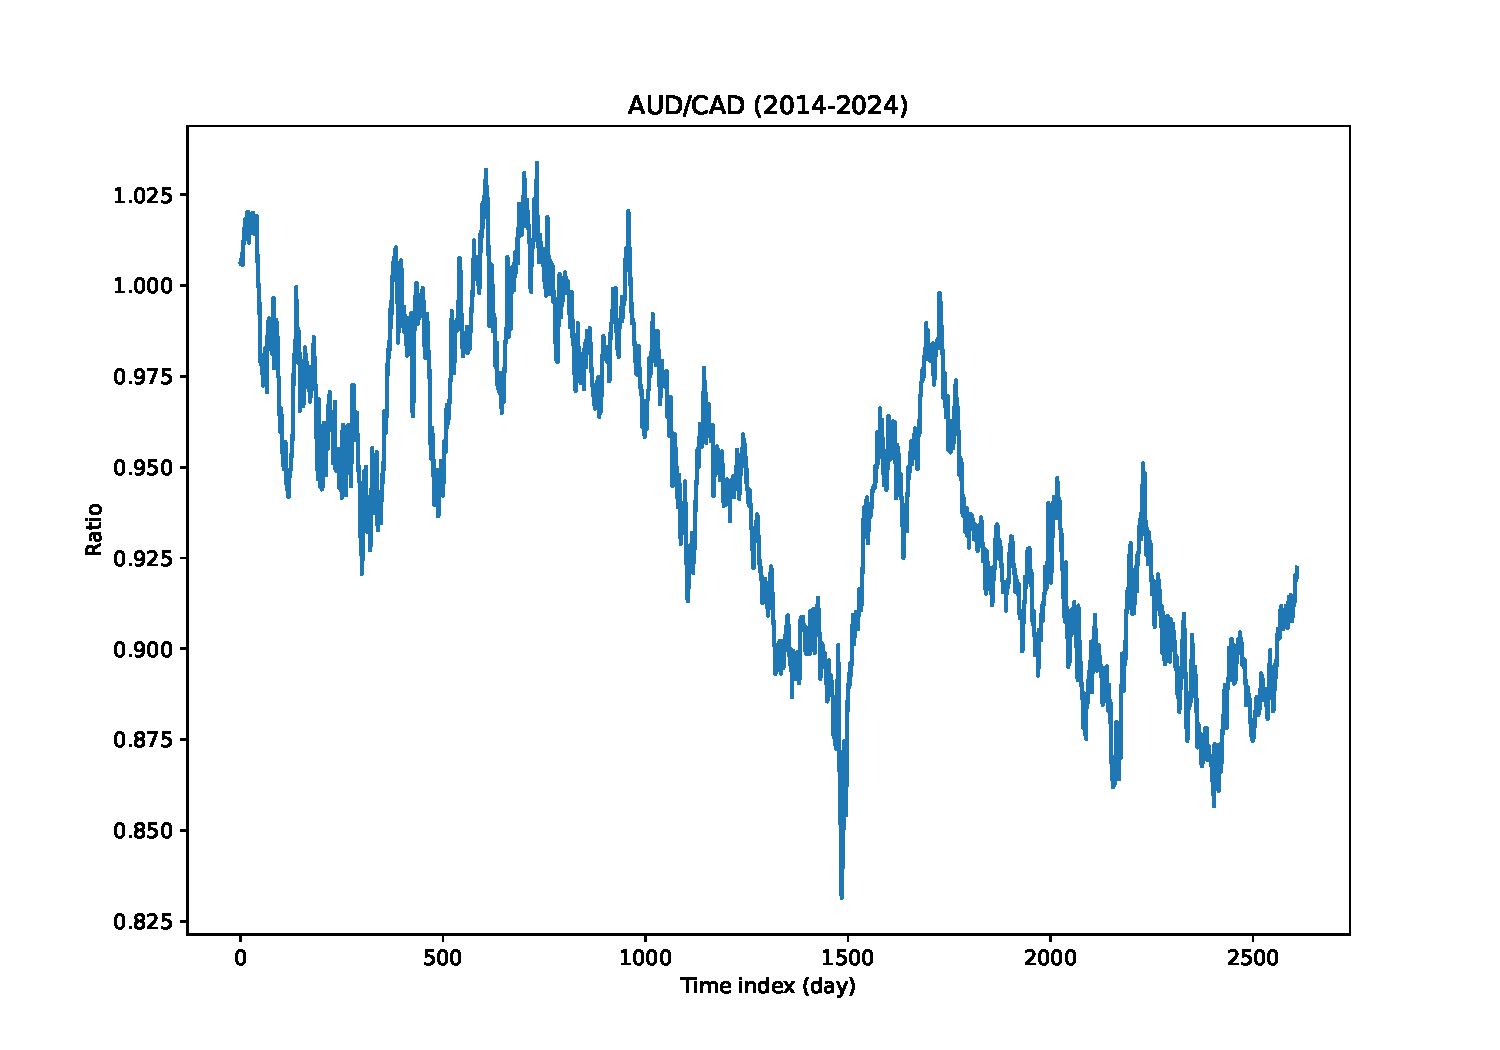
\includegraphics[witdth=\linewidth]{./img/meo.pdf}
%   % \caption{This is a caption \cite{challu2023nhits}}
% \end{figure}

\begin{figure}
  \centering
  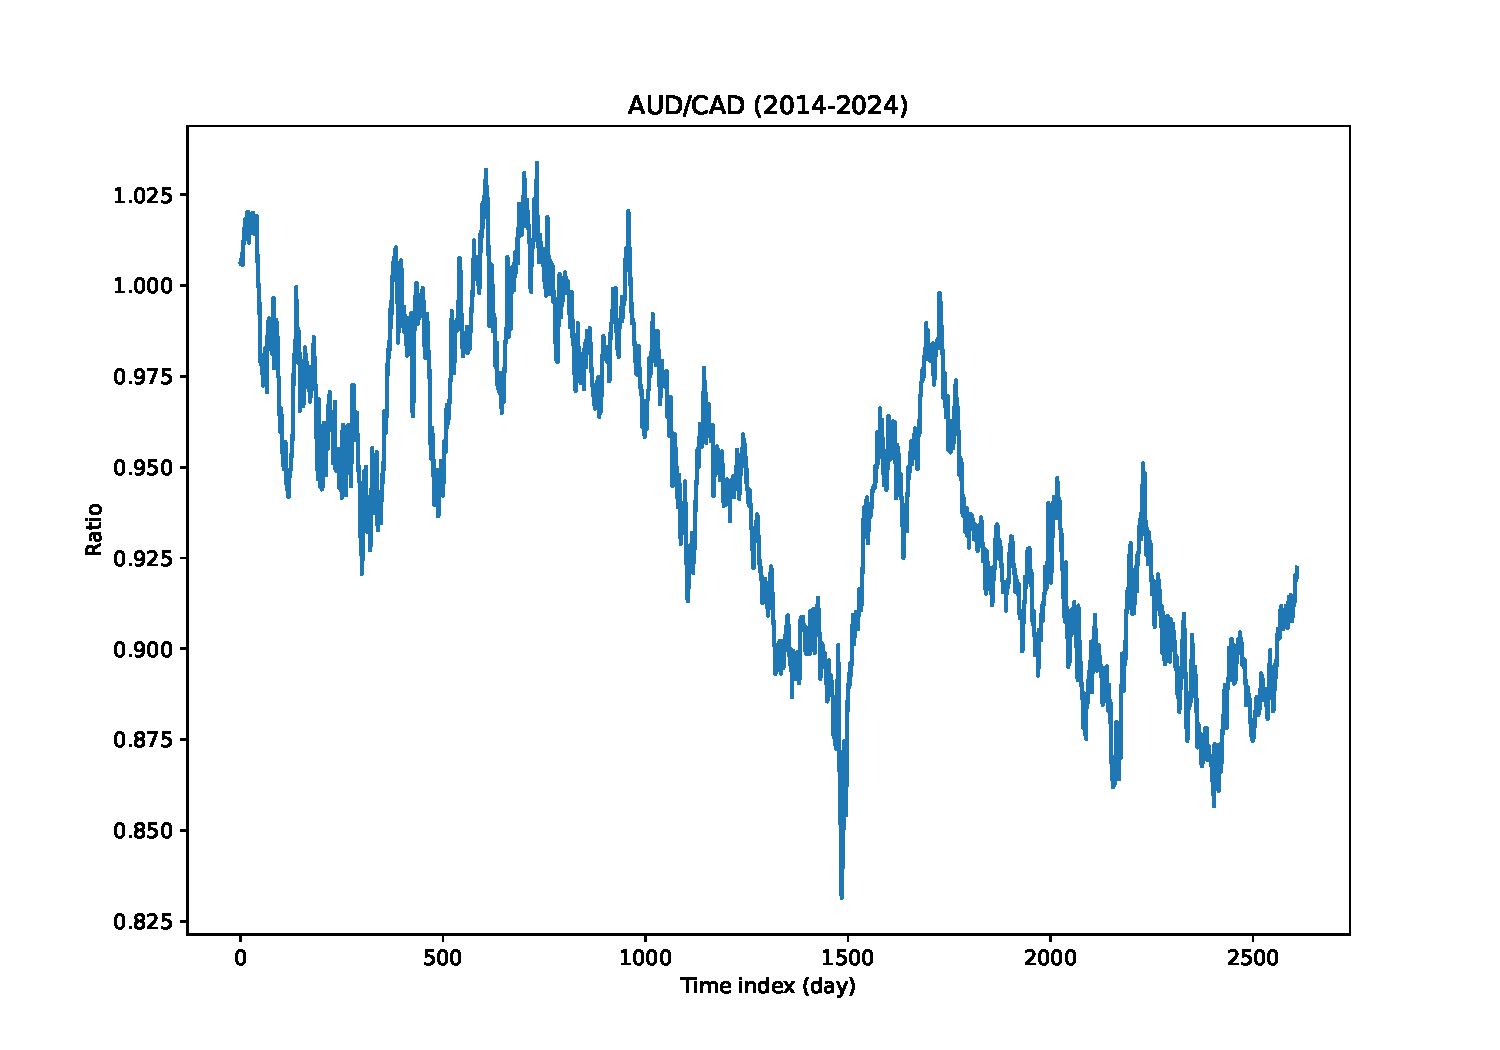
\includegraphics[width=\linewidth]{img/meo.pdf}
  \caption{Your figure caption here.}
  \label{fig:your-label}
\end{figure}

% \mathbf{y}_{t-L:t, l+1} &= \mathbf{y}_{t-L:t, l} - \mathbf{\hat{y}}_{t+1:t+H, l}

% nói về ưu điểm, nhược điểm của fundamental analysis and technical analysis --> đây là nói chung, sẽ có phần nói riêng sau (nói về từng phương pháp, dẫn đến phương pháp của tôi)

% tình hình kinh tế, chính trị, những thứ khó có thể cấu trúc hóa thành dữ liệu cho máy học.

%----------------------------------------
% \newcommand{\scale}{0.48}
% \begin{figure}[htbp]
%   \large
%   \centering
%   (a) I-type stacking of insulating TR lattice \\
%   \begin{minipage}{\scale\hsize}
%     \includegraphics[width=\hsize]{tri_off_top.eps}
%   \end{minipage}
%   \begin{minipage}{\scale\hsize}
%     \includegraphics[width=\hsize]{tri_off_side.eps}
%   \end{minipage}

% 	\vspace{5mm}
%   (b) II-type stacking of insulating TR lattice \\
%   \begin{minipage}{\scale\hsize}
%     \includegraphics[width=\hsize]{tri_on_top.eps}
%   \end{minipage}
%   \begin{minipage}{\scale\hsize}
%     \includegraphics[width=\hsize]{tri_on_side.eps}
%   \end{minipage}

% \vspace{5mm}
%   (c) I-type stacking of metallic NTR lattice \\
%   \begin{minipage}{\scale\hsize}
%     \includegraphics[width=\hsize]{ntr_off_top.eps}
%   \end{minipage}
%   \begin{minipage}{\scale\hsize}
%     \includegraphics[width=\hsize]{ntr_off_side.eps}
%   \end{minipage}

% \vspace{5mm}
%   (d) II-type stacking of metallic NTR lattice \\
%   \begin{minipage}{\scale\hsize}
%     \includegraphics[width=\hsize]{ntr_on_top.eps}
%   \end{minipage}
%   \begin{minipage}{\scale\hsize}
%     \includegraphics[width=\hsize]{ntr_on_side.eps}
%   \end{minipage}
%   \caption{\ghost{fig.str}\label{fig.str}
%     Structure models of LiV$X_2$ (X = O, S, and Se).
%     The left figure is top-view and the right figure is side-view.
%     The green balls are Li, the blue balls are V, and red balls are O.
%   }
% \end{figure}
%----------------------------------------

%%%%%%%%%%%%%%%%%%%%%%%%%%%%%%%%%%%%%%%%%%%%%%%%%%%
\section{Methodology}
\label{sec.method}
%%%%%%%%%%%%%%%%%%%%%%%%%%%%%%%%%%%%%%%%%%%%%%%%%%%
Fixed-node DMC

\vspace{2mm}
Fixed-node DMC
%----------------------------------------
\begin{equation}
\left[\sum_j\frac{1}{2}\nabla^2_j
+ V_{\rm MB}\left(\vec R\right)
\right]\Psi\left(\vec R\right)
= E~\Psi\left(\vec R\right) \ .
\end{equation}
%----------------------------------------
Fixed-node DMC

%----------------------------------------
\begin{equation}
\left[\cfrac{1}{2}~\nabla^2_j
+ v_{\rm ext}\left(\vec r_j\right)
+ v_{\rm XC}\left(\vec r_j\right)
\right]\psi\left(\vec r_j\right)
= \varepsilon~\psi\left(\vec r_j\right) \ .
\end{equation}
%----------------------------------------
Fixed-node DMC

\vspace{2mm}
Fixed-node DMC
%----------------------------------------
\begin{align}
  E\left[\Psi_T\right]
  &=\frac{\int d\vec{R}\cdot \Psi_T^*\left(\vec{R}\right)
  \hat{H}\Psi_T\left(\vec{R}\right)}{\int d\vec{R}\cdot \Psi_T^*\left(\vec{R}\right)\Psi_T\left(\vec{R}\right)} ,
  \label{eq.varfunc}
\end{align}
%----------------------------------------
\ghost{eq.varfunc}
Fixed-node DMC

\vspace{2mm}
Fixed-node DMC

\vspace{2mm}
Fixed-node DMC

%%%%%%%%%%%%%%%%%%%%%%%%%%%%%%%%%%%%%%%%%
\section{Experiment}
\label{sec.experiment}
%%%%%%%%%%%%%%%%%%%%%%%%%%%%%%%%%%%e%%%%%%
\subsection{Density functional theory}
Density functional theory

\subsection{Fixed--node DMCTEXT}
Fixed--node DMCTEXT

\vspace{2mm}
Fixed--node DMCTEXT

\vspace{2mm}
Fixed--node DMCTEXT

%%%%%%%%%%%%%%%%%%%%%%%%%%%%%%%%%%%%%%%%%%%%%%%%
\section{Results and discussion}
\label{sec.results}
%%%%%%%%%%%%%%%%%%%%%%%%%%%%%%%%%%%%%%%%%%%%%%%%
Results and discussion

%----------------------------------------
% \begin{figure}[htbp]
%   \centering
%   \includegraphics[width=\hsize]{all.eps}
%   \caption{\ghost{fig.all}\label{fig.all}
% 	FNDMC and DFT results of relative energies of
% 	the four candidate structures of LiV$X_2$
% 	(X = O, S, and Se):
% 	the I- and II-type stacking of the insulating
%     TR and metallic NTR lattices.
% 	Their structures are shown in Figure \ref{fig.str}.
% 	The lowest energy among the four structures is set
% 	to be zero and the others are given as relative values
% 	from the lowest energy.
%   }
% \end{figure}
%----------------------------------------

\vspace{2mm}
Results and discussion

\vspace{2mm}
Results and discussion

%%%%%%%%%%%%%%%%%%%%%%%%%%%%%%%%%%%%%%%%%
\section{Conclusion}
\label{sec.conc}
%%%%%%%%%%%%%%%%%%%%%%%%%%%%%%%%%%%%%%%%%
Conclusion

% We also compared DFT results using PBE\cite{PBE}, optPBE-vdW-DF\cite{2009JK_AM,vdW-DFa,vdW-DFb}, SCAN\cite{SCAN}, and HSE06\cite{HSE06} functionals with the FNDMC results. All of them also favour non-trimerized structures in all three materials, but none of the DFT functionals do not quantitatively agree with FNDMC. Thus our results demonstrate that this series of materials: LiVO$_2$,  LiVS$_2$, and LiVSe$_2$ represent a real challenge for computational schemes and also motivates further experimental study of the ground state properties of LiVSe$_2$.

%%%%%%%%%%%%%%%%%%%%%%%%%%%%%%%%%%%%%%%%%
\section{Acknowledgements}
%%%%%%%%%%%%%%%%%%%%%%%%%%%%%%%%%%%%%%%%%
The work was carried out within the state assignment of Ministry of Science and Higher Education of the Russian Federation (No. AAAA-A18-118020190095-4, topic ``Quantum''). G.I.P is grateful for financial supports from JST SPRING, Grant Number JPMJSP2102. K. H. is grateful for financial support from MEXT-KAKENHI (JP19K05029, JP21K03400, JP21H01998, and JP22H02170). R.M. is grateful for financial supports from MEXT-KAKENHI (22H05146, 21K03400 and 19H04692).

%%%%%%%%%%%%%%%%%%%%%%%%%%%%%%%%%%%%%%%%%
\section{Author contributions}
%%%%%%%%%%%%%%%%%%%%%%%%%%%%%%%%%%%%%%%%%
All authors contributed to conceiving the idea. T.I., A.V.U, and G.I.P performed the calculations. T.I. made the all figures. R.M and S.V.S supervised the work. All authors contributed to the discussion and writing of the paper.

%%%%%%%%%%%%%%%%%%%%%%%%%%%%%%%%%%%%%%%%%
\section{Data availability statement}
%%%%%%%%%%%%%%%%%%%%%%%%%%%%%%%%%%%%%%%%%
The datasets used and/or analyzed during the current study available from the corresponding authors on reasonable request.

%%%%%%%%%%%%%%%%%%%%%%%%%%%%%%%%%%%%%%%%%
\bibliographystyle{elsarticle-harv} 
\bibliography{references}
\end{document}
%%%%%%%%%%%%%%%%%%%%%%%%%%%%%%%%%%%%%%%%%



%%%%%%%%%%%%%%%%%%%%%%%%%%%%%%%%%%%%%%%%%%
%\section{Appendix}
%%%%%%%%%%%%%%%%%%%%%%%%%%%%%%%%%%%%%%%%%%
%We used the VASP code\cite{VASP} for the calculations explained in this appendix.
%We relaxed the four structures of Figure \ref{fig.str}
%for every LiV$X_2$ ($X$ = O, S, and Se) with each of PBE\cite{PBE},
%optPBE-vdW-DF\cite{2009JK_AM,vdW-DFa,vdW-DFb}, and HSE06\cite{HSE06} functionals.
%We evaluated the relative energies of structures relaxed by every functional by PBE-DFT.
%%as shown in Figure \ref{fig.geomErr}.
%We found that the differences of the relative energies
%among the structures relaxed by different functionals are at most 0.018 eV/f.u.
%%the differences of the time-series in Figure \ref{fig.geomErr} are within 0.018 eV/f.u.

%%----------------------------------------
%\begin{figure}[htbp]
%  \centering
%  \includegraphics[width=\hsize]{geomErr.eps}
%  \caption{\ghost{fig.geomErr}\label{fig.geomErr}
%    FNDMC and DFT results of relative energies of the four candidate structures
%    of LiV$X_2$ (X = O, S, and Se).
%    The candidate structures are shown in Figure \ref{fig.str}.
%    TR-I and TR-II (left from the vertical line) are trimmerized
%    and NTR-I and NTR-II (right from the vertical line) are
%    non-trimmerized structures, respectively.
%    FNDMC results are same as Figure \ref{fig.dmconly}.
%    The lowest energy among the four structures is set to be zero
%    and the others are given as relative values from the lowest energy.
%  }
%\end{figure}
%%----------------------------------------
